\newpage
\hypertarget{initialize notes}{}
\subsection{A short note on the \texttt{initializeBox} method}
\genHeader

Pretend you've just updated the control flow in your \texttt{grow} SDM, and haven't specified \texttt{initializeBox} yet. After saving and building, you will be
able to see the changes in \texttt{BoxImpl.java}, the source file containing the generated code. In fact, open this file now and navigate to \texttt{grow},
which starts at (approximately) line 207 (Fig.~\ref{eclipse:initBoxImpl}). This is the generated \emph{statement node} code and, as you can see, all it does is
invoke your method and branch based on its result. 

\begin{figure}[htp]
\begin{center}
  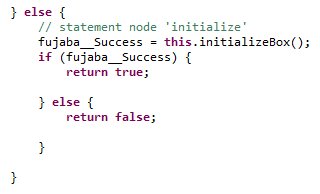
\includegraphics[width=0.5\textwidth]{eclipse_boxImplStatementNode}
  \caption{Code generated for branching with a statement node}
  \label{eclipse:initBoxImpl}
\end{center}
\end{figure}

Hold \texttt{Ctrl} while clicking on \texttt{initializeBox()} to automatically
jump to its declaration.
If you didn't complete the SDM, it would look like Fig.~\ref{eclipse:initBoxDecl}.

\begin{figure}[htp]
\begin{center}
  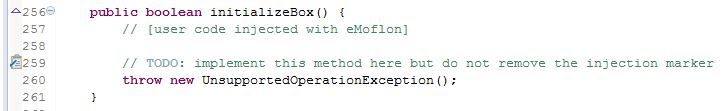
\includegraphics[width=\textwidth]{eclipse_initializeBoxDeclaration}
  \caption{The \texttt{initializeBox} declaration}
  \label{eclipse:initBoxDecl}
\end{center}
\end{figure}

You have the choice of either implementing the method by hand here in Java as an injection, or you can return to the metamodel and implement it there as an SDM.
The statement node will work just fine in both cases.

Using Java and injections makes sense if the method is non-structural, but seeing as we must check to see if there is a single partition, then create the
first two partitions of the box if it succeeds, \texttt{initializeBox} is actually quite structural and can be described beautifully as a pattern. This is why
we opted to specify it as an SDM.

